\documentclass[10pt,letterpaper]{article}

\usepackage{cogsci}
\usepackage{pslatex}
\usepackage{apacite}
\usepackage{graphicx}

\title{Memory Driven Temporal Preparation: A Cognitive Model}
 
\author{{\large \bf Steven Bosch (s1861948)} \\
  Faculty of Mathematics and Natural Sciences}


\begin{document}
\maketitle

\begin{abstract}
Blabla

\textbf{Keywords:} 
temporal preparation; cue target interval timing; Hazard function; long term memory
\end{abstract}

\section{Introduction}
The human brain has many traits that we are hardly aware of during our everyday lives, even though these traits have a great impact on our experiences and actions. One such trait is the ability of cue target interval timing. Both consciously and unconsciously this ability is exercised in numerous situations, such as waiting for traffic lights, expecting a sound when something falls or simply expecting the second hand of a clock to move to the next second. What are the cognitive mechanisms behind this ability?

One theory encompasses the \textit{Hazard function}. This function describes that the conditional probability of the occurrence of a target event after the presentation of a cue increases over time given that the event has not yet occurred. While this function has been successfully used to predict interval timing behaviour \cite{Nobre, Vangkilde}, it does not provide an explanation as to the cognitive processes behind it. Moreover it does not take into account memory traces of preceding timing experiences. The past years research began on this basis \cite{Los1, Howard, Taatgen}. Los et al. (2014) developed what they called the \textit{multiple trace theory of temporal preparation} (MTP), in which every new trial causes a memory trace to be created, storing a temporal profile of that trial.This memory trace subsequently contributes to the preparation of subsequent trials. 

A recent experiment by Los et al. indicated that temporal preparation is indeed driven by memory \cite{Los2}. In the experiment different groups of participants were presented with different distributions of foreperiods between temporal cues and target stimuli. Three of these experiments showed a transfer effect of this manipulation in a test phase where all participants received the same uniform distribution, indicating memory influence. 

This paper discusses a model that tries to capture (some of) the cognitive processes behind the phenomenon that the experiment by Los et al. (2015) brought to light. Using a cognitive model might give us more insight into he workings of this particular cognitive process.

\section{Experiment}
\subsection{Method}
In Los et al.'s (2015) experiment sixty-four students were randomly assigned to one of two groups, each consisting of 32 participants. The participants were asked to sit behind a computer screen with their left index finger on the \textit{z} key and their right index finger on the \textit{m} key. Each trial started with the appearance of a black plus sign, \textit{S1}, in the middle of the screen. Subsequently after a given foreperiod of either 400, 800, 1200 or 1600 ms a second signal, \textit{S2}, appeared. Seeing the signal, the participants had to press either \textit{z}, when \textit{S2} appeared left, or \textit{m} when \textit{S2} appeared right. They were instructed to perform this action as fast as they could. After the response the screen turned black and after an interval of 1.5 seconds the next trial would start.

Every participant had to complete 5 blocks of 120 trials each. The distribution of trials within a block was either uniform (30 trials of each foreperiod), exponential (64, 32, 16 and 8 trials for foreperiods of 400, 800, 1200 and 1600 ms respectively) or anti-exponential (8, 16, 32 and 64 trials for foreperiods of 400, 800, 1200 and 1600 ms respectively) distribution. Table \ref{Table1} shows the foreperiod distributions of the blocks per group. For both of the groups block 1, 4 and 5 were uniform, whereas block 2 and 3 were either exponential or anti-exponential.

In the experiment the participants were informed every block about their mean response time (RT) and the percentage of correct responses of that block. Furthermore after block 3 they were informed of the distributions of the preceding and succeeding two blocks.

\begin{table}
	\centering
	\caption{Successive foreperiod distributions across blocks for group 1 and 2 (Uni \= uniform, Exp \= exponential, Anti-exp \= anti-exponential).}
	\begin{tabular}{c|c|c|c|c|c}
		Block & 1 & 2 & 3 & 4 & 5 \\
		\hline
		Group 1 & Uni & Exp & Exp & Uni & Uni \\
		Group2 & Uni & Anti-exp & Anti-exp & Uni & Uni
	\end{tabular}
	\label{Table1}
\end{table}

\subsection{Results}
Figure \ref{LosFigure} shows the results of Los et al.'s experiment. The figure shows that for the first uniform distribution, when the participants do not have any prior experience with the experiment yet, their mean RT fore a foreperiod of 400 ms is around 360 ms. It decreases exponentially to around 320 ms for a foreperiod of 1600. In blocks 2 and 3 we see a clear difference between the exponential and anti-exponential distribution. The mean RT for the exponential group decreases greatly for shorter foreperiods to almost the same level of the longer foreperiods, while the opposite happens for the anti-exponential group: the mean RTs increase, most of all for the shorter foreperiods. In the final two blocks we can still see slight remnants of the preceding distributions, with slight differences being there between the two groups of participants.

As discussed in the introduction, it appears the cognitive process of cue target interval timing involves more than just the hazard function. Indeed, otherwise there would have been no difference between the mean RTs of different foreperiod distributions.

\begin{figure}
	\centering
	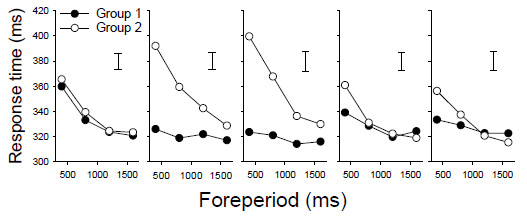
\includegraphics[width=\columnwidth]{Los1.png}
	\caption{Los et al.'s experiment results of mean response time as a function of group, block and foreperiod. Illustration from Los et al. (2015).}
	\label{LosFigure}
\end{figure}

\section{Model}
\subsection{Method}
\subsection{Results}



\begin{figure}
	\centering
	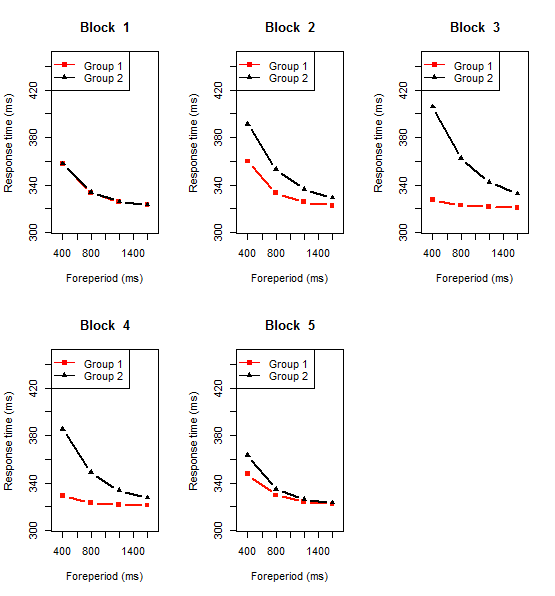
\includegraphics[width=\columnwidth]{5blocks2.png}
	\caption{Model results of mean response time as a function of group, block and foreperiod.}
	\label{5blocks}
\end{figure}

\section{Discussion}



\bibliographystyle{apacite}
\setlength{\bibleftmargin}{.125in}
\setlength{\bibindent}{-\bibleftmargin}
\bibliography{bibliography}

\end{document}
